\documentclass[tikz,border=2pt]{standalone}
\renewcommand{\familydefault}{\sfdefault}
\usetikzlibrary{arrows.meta,calc,positioning}
\tikzset{every picture/.style={line width=1pt, >=Stealth},
         hl/.style={fill=black, fill opacity=0.12, text opacity=1}}
\begin{document}
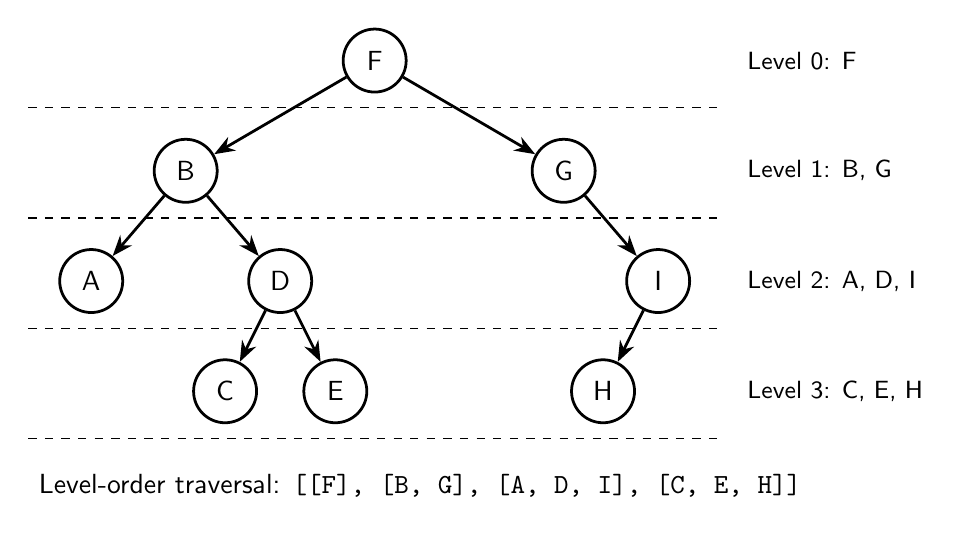
\begin{tikzpicture}[tn/.style={draw, circle, minimum size=0.8cm, inner sep=0pt},
    cell/.style={draw, minimum size=0.75cm}]
  % The same binary tree is used for every traversal on this page.
  \foreach \n/\x/\y in {F/0/0, B/-2.4/-1.4, G/2.4/-1.4, A/-3.6/-2.8, D/-1.2/-2.8, I/3.6/-2.8, C/-1.9/-4.2, E/-0.5/-4.2, H/2.9/-4.2}
    \node[tn] (\n) at (\x, \y) {\n};
  \foreach \a/\b in {F/B, F/G, B/A, B/D, D/C, D/E, G/I, I/H} \draw[->] (\a) -- (\b);

  % Each level is one batch of the queue, visited left to right.
  \foreach \lvl/\y/\nodes in {0/0/{F}, 1/-1.4/{B, G}, 2/-2.8/{A, D, I}, 3/-4.2/{C, E, H}} {
    \draw[thin, dashed] (-4.4, \y - 0.6) -- (4.4, \y - 0.6);
    \node[anchor=west, font=\small] at (4.6, \y) {Level \lvl: \nodes};
  }
  \node[anchor=west] at (-4.4, -5.4) {Level-order traversal: \texttt{[[F], [B, G], [A, D, I], [C, E, H]]}};
\end{tikzpicture}
\end{document}
